\color{black}
\section{Evaluation}

\label{sec:evaluation}
The aim of our experimental study is three-fold:
\begin{enumerate}
    \item Check whether there exists a universal pipeline prototype that works best for any classification problem considered  (i.e., dataset and ML algorithm) (Section~\ref{sec:eval-universal-pipeline}).
    \item Assess and compare the performance of the effective pipelines constructed using our method against the set of exhaustively generated pipeline prototypes (Section~\ref{sec:eval-our-vs-rest}).
    \item Assess and compare the impact of dedicating a portion of the optimization time to the effective pipelines constructed using our method, with the impact of using the whole optimization time for the hyper-parameters of the ML algorithm (Section~\ref{sec:eval-dpso-vs-cash}).
\end{enumerate}

The experiments were performed on an Intel Core i7 machine with 12 cores, running at 3.20 GHz with 64 GB of main memory. As a platform for running the SMBO optimization algorithm we use HyperOpt. Furthermore, the datasets used in the experiments are the ones from the OpenML repository (see Section~\ref{sec:rules-learned:algorithm}). Finally, the classification algorithms considered are \textit{NB}, \textit{KNN}, and \textit{RF}. All the experiments for a single algorithm, on average took approximately two weeks\footnote{The source code and the datasets for reproducing the experiments can be found in 
\href{https://github.com/josephgiovanelli/effective\_preprocessing\_pipeline\_evaluation}{https://github.com/josephgiovanelli/effective\_preprocessing\_pipeline\_evaluation}}.

\subsection{Universal pipeline prototype}
\label{sec:eval-universal-pipeline}
The goal of this experiment is to demonstrate the difficulty of blindly finding the right pipeline prototype (i.e., without considering any meaningful or promising precedence).
In Table~\ref{tbl:pipeline-enumeration}, we list the exhaustive set of pipeline prototypes generated considering the compatible precedence graph in Table~\ref{tbl:rules}a (i.e., 24 compatible permutations). In a real scenario, this number would be too high for splitting the time budget in order to optimize them. 
Yet, for the sake of this experiment, we exhaustively optimize all the prototypes, for each dataset. Thus, for each pipeline prototype and for each dataset, the SMBO algorithm is configured to assign a 200 seconds time budget to the phase of instantiating and optimizing the pipeline prototype, and another 200 seconds to the phase of optimizing the hyper-parameters of the ML algorithm.

\begin{table}[t]
\caption[Enumeration of the pipelines that can be generated by compatible precedence]{Exhaustive set of pipeline prototypes generated using the compatible precedence graph of Table~\ref{tbl:rules}a. $E$ - Encoding; $N$ - Normalization; $D$ - Discretization; $I$ - Imputation; $R$ - Rebalancing; $F$ - Feature Engineering.
}
\footnotesize
\label{tbl:pipeline-enumeration}
\begin{center}
\begin{tabular}{@{}lllll@{}}
\toprule
ID & Pipeline prototype & ID & Pipeline prototype                                                                   \\ \toprule
1  & {\color[HTML]{000000} $I\veryshortarrow E\veryshortarrow N \veryshortarrow D\veryshortarrow F \veryshortarrow R$} & 13 & {\color[HTML]{000000} $I\veryshortarrow E \veryshortarrow F \veryshortarrow N \veryshortarrow D\veryshortarrow R$} \\
2  & {\color[HTML]{000000} $I\veryshortarrow E\veryshortarrow N \veryshortarrow D\veryshortarrow R \veryshortarrow F$} & 14 & {\color[HTML]{000000} $I\veryshortarrow E \veryshortarrow F \veryshortarrow N \veryshortarrow R \veryshortarrow D$} \\
3  & {\color[HTML]{000000} $I\veryshortarrow E\veryshortarrow N \veryshortarrow F \veryshortarrow D\veryshortarrow R$} & 15 & {\color[HTML]{000000} $I\veryshortarrow E \veryshortarrow F \veryshortarrow D\veryshortarrow N \veryshortarrow R$} \\
4  & {\color[HTML]{000000} $I\veryshortarrow E\veryshortarrow N \veryshortarrow F \veryshortarrow R \veryshortarrow D$} & 16 & {\color[HTML]{000000} $I\veryshortarrow E \veryshortarrow F \veryshortarrow D\veryshortarrow R \veryshortarrow N$} \\
5  & {\color[HTML]{000000} $I\veryshortarrow E\veryshortarrow N \veryshortarrow R \veryshortarrow D\veryshortarrow F$} & 17 & {\color[HTML]{000000} $I\veryshortarrow E \veryshortarrow F \veryshortarrow R \veryshortarrow N \veryshortarrow D$} \\
6  & {\color[HTML]{000000} $I\veryshortarrow E\veryshortarrow N \veryshortarrow R \veryshortarrow F \veryshortarrow D$} & 18 & {\color[HTML]{000000} $I\veryshortarrow E \veryshortarrow F \veryshortarrow R \veryshortarrow D\veryshortarrow N$} \\
7  & {\color[HTML]{000000} $I\veryshortarrow E \veryshortarrow D\veryshortarrow N \veryshortarrow F \veryshortarrow R$} & 19 & {\color[HTML]{000000} $I\veryshortarrow E \veryshortarrow R \veryshortarrow N \veryshortarrow D \veryshortarrow F$} \\
8  & {\color[HTML]{000000} $I\veryshortarrow E \veryshortarrow D\veryshortarrow N \veryshortarrow R \veryshortarrow F$} & 20 & {\color[HTML]{000000} $I\veryshortarrow E \veryshortarrow R \veryshortarrow N \veryshortarrow F \veryshortarrow D$} \\
9  & {\color[HTML]{000000} $I\veryshortarrow E \veryshortarrow D\veryshortarrow F\veryshortarrow N \veryshortarrow R$} & 21 & {\color[HTML]{000000} $I\veryshortarrow E \veryshortarrow R \veryshortarrow D\veryshortarrow N \veryshortarrow F$} \\
10 & {\color[HTML]{000000} $I\veryshortarrow E \veryshortarrow D\veryshortarrow F \veryshortarrow R\veryshortarrow N$} & 23 & {\color[HTML]{000000} $I\veryshortarrow E \veryshortarrow R \veryshortarrow D \veryshortarrow F \veryshortarrow N$} \\
11 & {\color[HTML]{000000} $I\veryshortarrow E \veryshortarrow D\veryshortarrow R \veryshortarrow N \veryshortarrow F$} & 23 & {\color[HTML]{000000} $I\veryshortarrow E \veryshortarrow R \veryshortarrow F \veryshortarrow N \veryshortarrow D$} \\
12 & {\color[HTML]{000000} $I\veryshortarrow E \veryshortarrow D\veryshortarrow R \veryshortarrow F\veryshortarrow N$} & 24 & {\color[HTML]{000000} $I\veryshortarrow E \veryshortarrow R \veryshortarrow F \veryshortarrow D\veryshortarrow N$}
\\ \bottomrule
\end{tabular}
\end{center}
\end{table}

The results obtained are shown in Figure~\ref{fig:eval-universal-pipeline}.
The enumerated prototypes are listed in the ordinate axis and each stacked bar represents the percentage of cases for which that prototype achieved the best performance across different ML algorithms (the contribution of each algorithm is represented with a different color). In an ideal scenario, for a pipeline to be considered \textit{universal}, it should perform best in all or at least most of the cases, which is clearly not happening. Observe that, even the best performing pipeline is only the best in 19\% of the cases, which is obviously far from being \textit{universal}. Hence all (or at least several) pipelines need to be evaluated together, in order to obtain better solutions. 

\begin{figure}[t]
    \centering
    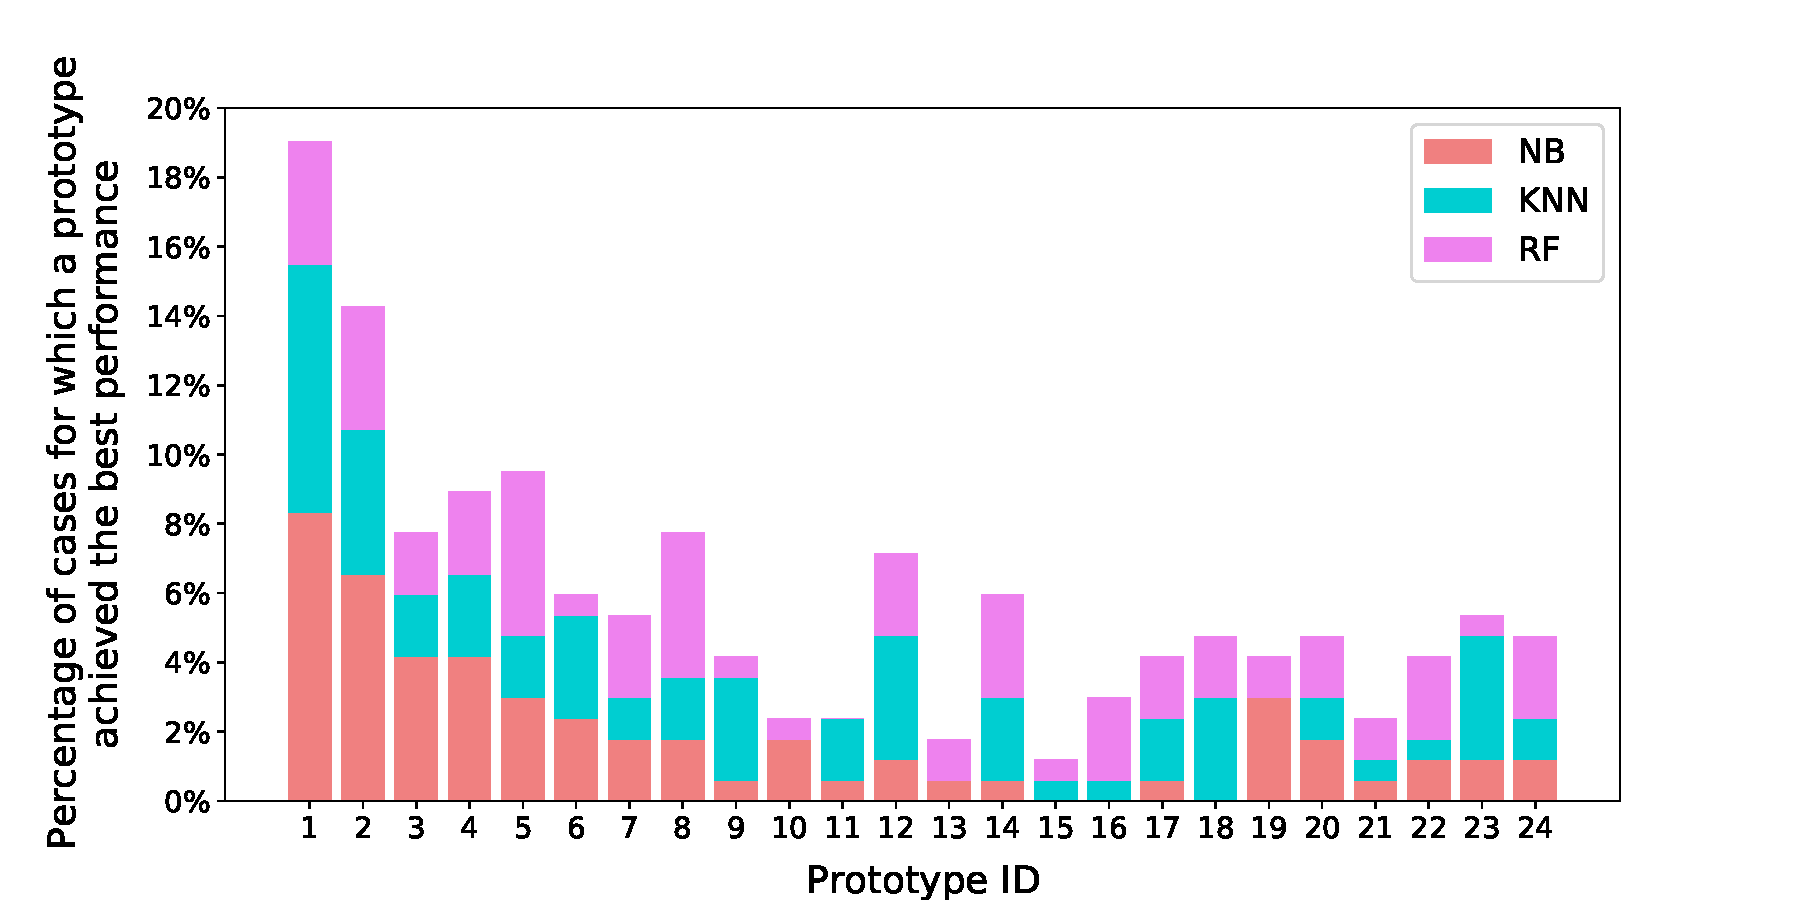
\includegraphics[width=0.8\textwidth]{figures/evaluation1.pdf}
    \caption{Comparison of the goodness of the exhaustive set of prototypes.}
    \label{fig:eval-universal-pipeline}
    %\besim{To be updated, start from \#1.}
\end{figure}

\subsection{Exhaustive versus effective prototypes}
\label{sec:eval-our-vs-rest}
Given that there is no single universal pipeline, one can opt for feeding all the possible prototypes (see Table~\ref{tbl:pipeline-enumeration}) to the optimization algorithm in order to get the best solutions out of them. 
%Even though this is probably infeasible in practice, for the sake of this experiment, on one hand, 
As before, we assign a budget of 200 seconds for the optimization of each prototype, hence 80 minutes in total for all the set of 24 \textit{exhaustive prototypes} in order to find the optimal pipeline for every dataset. On the other hand, we take only the five \textit{effective prototypes} resulting from the application of our method and assign just 40 seconds time budget for the optimization of each one of them, hence 200 seconds in total. With the aim of comparing the two, and thus roughly understanding how close we are to the optimal case, in both cases, we dedicated the same time budget (i.e., 200 seconds) for the phase of optimizing the hyper-parameters of the ML algorithm.
In order to evaluate how close the \textit{effective prototypes} are to the \textit{exhaustive ones}, we calculate the \textit{normalized distance} from the result to the optimum:

\begin{equation*}
    normalized\;distance = \frac{Acc(d_{e\!f\!f\!ective},a^*) - Acc(d,a)}{Acc(d_{exhaustive},a^*) - Acc(d,a)}
\end{equation*}

where, $Acc(d,a)$ is the baseline performance (i.e., predictive accuracy of the algorithm $a$ with default hyper-parameters over the original dataset $d$). $Acc(d_{e\!f\!f\!ective},a^*)$ is the accuracy of the optimized algorithm $a^*$ over the dataset $d_{e\!f\!f\!ective}$ transformed using the optimized instantiation of the effective set of prototypes (i.e., our approach). Finally, ~$Acc(d_{exhaustive},a^*)$ is the accuracy of the optimized algorithm $a^*$ over the dataset $d_{exhaustive}$ transformed using the optimized pipeline instantiation of the exhaustive set of prototypes. The subtraction by $Acc(d,a)$ is done with the aim of weighting the difficulty of a dataset, hence allowing for comparisons in terms of the gain in accuracy. To this end, the bigger the potential gain (denominator) is, the bigger the obtained gain (numerator) must be, for the latter to be relevant. 

The results obtained for every dataset and algorithm are shown as boxplots in Figure~\ref{fig:eval-exhaustive-vs-effective}. Observe that, most of the cases are very close to the results obtained using the exhaustive set, the median distances being 91.51\%, 93.13\%, 88.97\%, for NB, KNN, and RF, respectively. 
In general, in 75\% of the cases the chosen pipelines are above 80\%, and only few outliers are below 60\%. Curiously, in some cases, we outperform the results over the exhaustive set of pipelines, but this is due to the randomness of the optimization algorithm, which unless it is given an unrealistically high budget of time, is not capable of finding the true optimal solution. We discarded the option of assigning a larger budget since this was not practical considering the huge search space and the lack of any guarantee of improvement. 

To summarize, the experiment shows that with roughly 24 times less time budget, we can obtain results that are as good as 90\% in the median compared to the exhaustive ones. The raw results (i.e., without the normalized distances) can be found on the aforementioned github page.

\begin{figure}[!t]
    \centering
    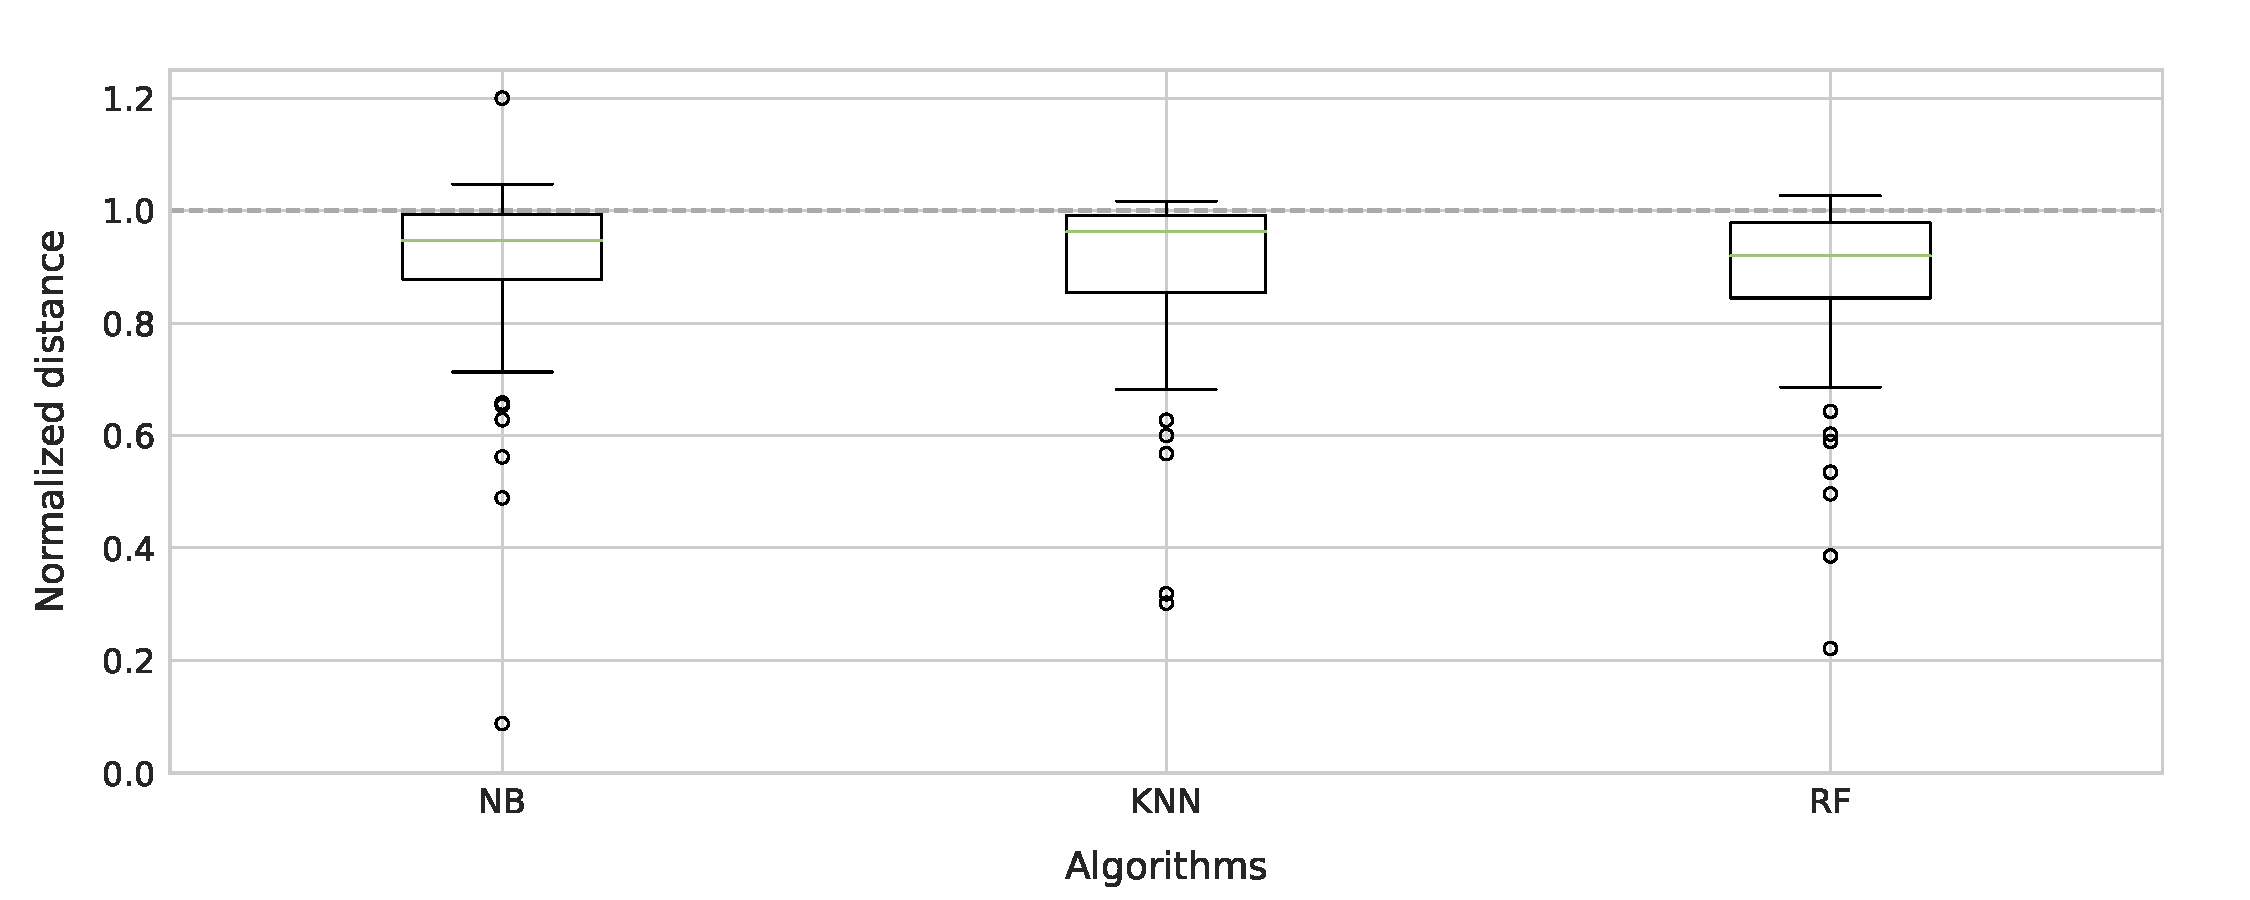
\includegraphics[width=0.7\textwidth]{figures/evaluation2.pdf}
    \caption{Normalized distances between the scores obtained by optimizing our effective prototypes and the ones obtained optimizing the exhaustive set.}
    \label{fig:eval-exhaustive-vs-effective}
\end{figure}

\subsection{Complementing hyper-parameter optimization with pre-processing}
\label{sec:eval-dpso-vs-cash}

\begin{figure*}[!t]
	\centering
	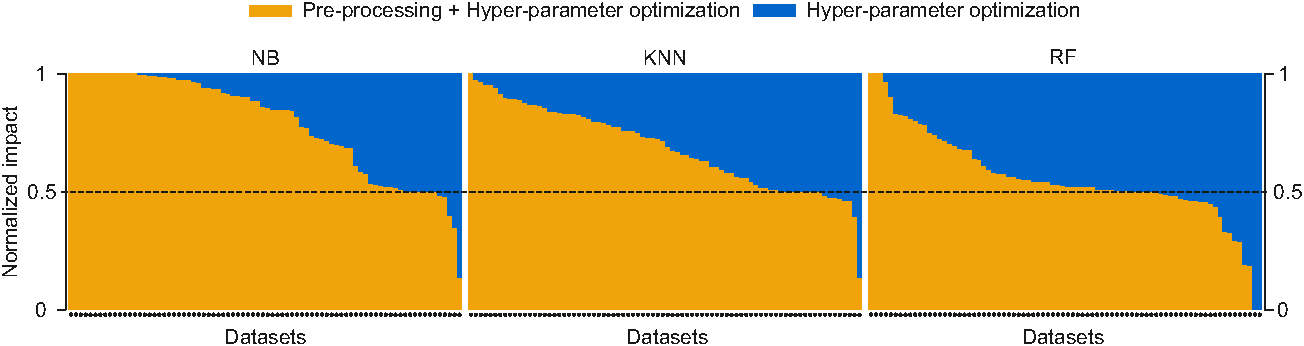
\includegraphics[width=1.0\textwidth]{figures/barplot-10.pdf}
	\caption{The impact of dedicating a portion of the optimization budget to pre-processing compared to using the whole optimization budget for the hyper-parameter optimization.}
	\label{fig:eval-pre-processing-hyper-parameter}
\end{figure*}

We have just shown that our effective pipeline prototypes have similar impact as the exhaustive prototypes. Now we want to compare the impact of effective prototypes against optimizing only the hyper-parameters of the ML algorithm. That is, we want to examine whether dedicating a part of the optimization budget to the pre-processing pipeline impacts more (positively) the results of the analysis, than using the whole budget for the hyper-parameter optimization\footnote{To enable the application of the ML algorithms on all the datasets, whenever required, we apply the necessary transformation (e.g, imputation or encoding).}. 

To this end, for the latter we now dedicate the total optimization budget (i.e., 400 seconds), and for the former, inspired by \cite{Quemy20InfSystems}, we split the budget 50-50 between the pre-processing pipeline optimization and the hyper-parameter optimization (i.e., 200 seconds for the pre-processing, and 200 seconds for the hyper-parameter optimization). The time for the pre-processing is further split among the five different pipeline prototypes (i.e., 40 seconds each).

To compare the results, we calculate the impact using the formulas below, that correspond to the normalized distance from either pre-processing or hyper-parameter optimization to the maximum improvement that can be achieved, regardless of whether pre-processing is applied or not. 

\begin{equation*}
    \text{\textit{pp impact}} = \frac{Acc(d_{e\!f\!f\!ective},a^*) - Acc(d,a)}{max(Acc(d_{e\!f\!f\!ective},a^*),Acc(d,a^*)) - Acc(d,a)}
\end{equation*}

\begin{equation*}
    \text{\textit{hp impact}} = \frac{Acc(d,a^*) - Acc(d,a)}{max(Acc(d_{e\!f\!f\!ective},a^*),Acc(d,a^*)) - Acc(d,a)}
\end{equation*}

where, $Acc(d,a)$ is the baseline accuracy (i.e., predictive accuracy of the algorithm $a$ with default hyper-parameters over the original dataset $d$). $Acc(d_{e\!f\!f\!ective},a^*)$ is the accuracy of the optimized algorithm $a^*$ over the dataset $d_{e\!f\!f\!ective}$ transformed using the optimized instantiation of the effective set of prototypes obtained using our method. Finally,  $Acc(d,a^*)$ is the accuracy of the optimized algorithm $a^*$ (i.e, using the entire budget) over the original dataset $d$.

To obtain relative values that sum to 1, we normalize the impacts dividing them by their sum. For instance, for the pre-processing score we calculate the following:
\begin{equation*}
    \text{\textit{normalized pp impact}} = \frac{\text{\textit{pp impact}}}
    {\text{\textit{pp impact}} + \text{\textit{hp impact}}}
\end{equation*}


We perform the same for the hyper-parameter impact and plot the results obtained for all the algorithms and datasets in Figure~\ref{fig:eval-pre-processing-hyper-parameter}, where each bar represents the results obtained for a single dataset. The different colors represent the impact values of pre-processing and hyper-parameter optimization. 

Observing the bar-charts one can see that (i) dedicating a portion of the budget to pre-processing, brings benefit to the analysis in most of the cases (i.e., $73\%$ of the cases), and (ii) the impact of hyper-parameter optimization, increases with the increase of the number of hyper-parameters of the ML algorithm (e.g., hyper-parameter optimization impacts more RF than NB). Overall, we can conclude that pre-processing is a critical step that once effectively applied may have a high positive impact on the final result of the analysis.